% Positive two-layer paper -- Korean internal-review source.
% 사용자가 최종 산출물을 요청하기 전에는 PDF/DOCX를 빌드하지 않는다.
\documentclass[12pt,a4paper]{article}
\usepackage[T1]{fontenc}
\usepackage[utf8]{inputenc}
\usepackage{kotex}
\usepackage[margin=25mm]{geometry}
\usepackage{amsmath,amssymb}
\usepackage{booktabs}
\usepackage{graphicx}
\usepackage[labelfont=bf,labelsep=period]{caption}
\usepackage{setspace}
\usepackage{fancyhdr}
\usepackage[hidelinks]{hyperref}
\setlength{\emergencystretch}{1em}
\setlength{\headheight}{14pt}
\onehalfspacing
\graphicspath{{pics/}}

\pagestyle{fancy}
\fancyhf{}
\fancyhead[R]{\small 두 표면 점군의 layer-first 재구성}
\fancyfoot[C]{\thepage}
\renewcommand{\headrulewidth}{0.4pt}

\title{서로 분리된 두 표면 점군의 Layer-First 재구성:\\
동결 합성 확인 실험과 Building-Disjoint S3DIS 검증}
\author{}
\date{}

\begin{document}
\maketitle
\thispagestyle{fancy}

\begin{abstract}
Alpha shape은 convex hull보다 오목한 경계와 분리된 성분을 잘 표현할 수
있지만, $\alpha$ 값을 바꾸는 것만으로는 가까이 있는 두 표면 사이의 잘못된
연결을 항상 막을 수 없다. 본 연구는 이 문제를 ``더 좋은 $\alpha$ 찾기''가
아니라 ``연결을 허용하기 전에 두 층을 먼저 구분하기''로 바꾼다. 입력은
레이블 없는 관측 XYZ 좌표뿐이다. 두 층을 관측 좌표로 추론하고, 층 분리가
불충분하면 fail-closed로 재스캔 또는 미지원 판정을 내리며, 통과한 경우에는
각 층을 고유한 접평면에서 따로 삼각분할한다. 144개 arbitrary-pose 합성
확인 사례에서 평균 F-score는 0.899로, PCA-anisotropic alpha의 0.516 및
weighted power-alpha의 0.620보다 높았고 모든 사례에서 승리했다. 합성
topology error는 각각 0, 45,606, 11,925였다. 한편 보정에 사용하지 않은
별도 건물의 S3DIS Area 5에서 자동 선정된 floor--ceiling 63개 방을 한 번만
열어 평가한 결과, 평균 F-score는 0.806 대 0.421 및 0.324였고 63/63
casewise 승리, topology error 0, 안전 수락 62/63을 얻었다. 실제 데이터에서
shared-trend 변형은 더 단순한 global-normal ablation과 같았다. 따라서
방어 가능한 긍정 결론은 충분히 평면적이고 겹치는 footprint를 가지며 간격이
긴 두 표면에서, observed-only routing과 층별 constrained connectivity가
anisotropic/weighted alpha보다 정확하고 topology가 안전하다는 것이다.
가까운 층, 교차 표면, outlier, 자동 semantic 추출 및 deployment는 주장하지
않는다.
\end{abstract}

\noindent\textbf{핵심어.} 점군 표면 재구성; alpha shape; constrained
connectivity; two-layer surface; fail-closed routing; S3DIS

\section{서론}

Alpha shape은 Delaunay triangulation의 일부 simplex를 스케일 $\alpha$에 따라
선택한다 \cite{edelsbrunner1994}. $\alpha$가 너무 작으면 표면에 구멍이
생기고, 너무 크면 빈 공간을 메우며 서로 떨어져 있어야 할 구조를 붙인다.
Density-scaled alpha와 normal-anisotropic alpha는 지역 점 밀도 또는 표면
방향을 반영해 이 문제를 줄인다 \cite{teichmann1998}. Weighted alpha는
regular triangulation을 사용하므로 연결성 자체도 바꿀 수 있다
\cite{edelsbrunner1992}. 그러나 이 방법들은 모두 두 표면의 합집합을 하나의
3차원 complex로 재구성한 뒤 어떤 cell을 남길지 결정한다.

두 표면이 같은 평면 footprint 위에 있지만 실제로는 서로 다른 층인 경우를
생각하자. Alpha complex에 두 층을 가로지르는 tetrahedron이나 triangle이
들어오면, $\alpha$를 줄여 그 cell을 제거하는 과정에서 필요한 층 내부 cell도
함께 잃을 수 있다. 이때 핵심 문제는 스케일만이 아니라 ``어떤 점끼리 연결할
수 있는가''이다.

본 연구는 입력 좌표에서 두 층을 먼저 추론한 뒤 각 층을 독립적으로
재구성하는 layer-first 원리를 검증한다(그림~\ref{fig:workflow-kr}). 후보
방법에는 semantic label, instance ID, 정답 layer, reference point 또는
baseline 결과를 주지 않는다. 방법은 공통 법선 방향과 두 개의 높이 mode를
추정하고, 관측 좌표에서 계산한 분리도와 sampling sufficiency가 동결 기준을
통과할 때만 결과를 허용한다. 통과한 두 point subset은 각각 PCA 접평면으로
투영한 후 2D Delaunay 삼각분할한다. 따라서 두 층을 가로지르는 face는 나중에
벌점을 받아 제거되는 것이 아니라 처음부터 후보가 될 수 없다.

검증은 두 단계다. 첫째, 결과 확인 전에 protocol과 gate를 고정한 144개
합성 Phase 50 panel에서 arbitrary 3D pose, 여섯 종류의 non-outlier stress,
강한 B5 PCA-anisotropic alpha 및 M1 weighted power-alpha comparator를
평가한다. 둘째, 실제 indoor scan point cloud인 S3DIS
\cite{armeni2016}에서 Areas 1/2/3/4/6만으로 corpus eligibility를 고정하고,
별도 건물인 Area 5를 protocol과 evaluator commit 뒤에 한 번만 연다. 이
실험은 floor와 ceiling annotation을 이용해 평가 corpus를 추출하지만,
재구성 후보는 결합된 XYZ만 받는다.

두 confirmatory panel 모두에서 후보는 B5와 M1을 모든 사례에서 이겼고
aggregate topology error가 0이었다. 그러나 실제 floor--ceiling panel에서
shared-quadratic trend와 단순 global-normal 모델은 같은 결과를 냈다. 그러므로
본 논문의 novelty는 PFTF, local-SPD metric 또는 shared-trend 우월성이 아니다.
Novelty는 관측 기반 fail-closed 두 층 routing과 연결성 제한을 하나의
검증된 재구성 절차로 결합한 데 있다.

\begin{figure}[t]
  \centering
  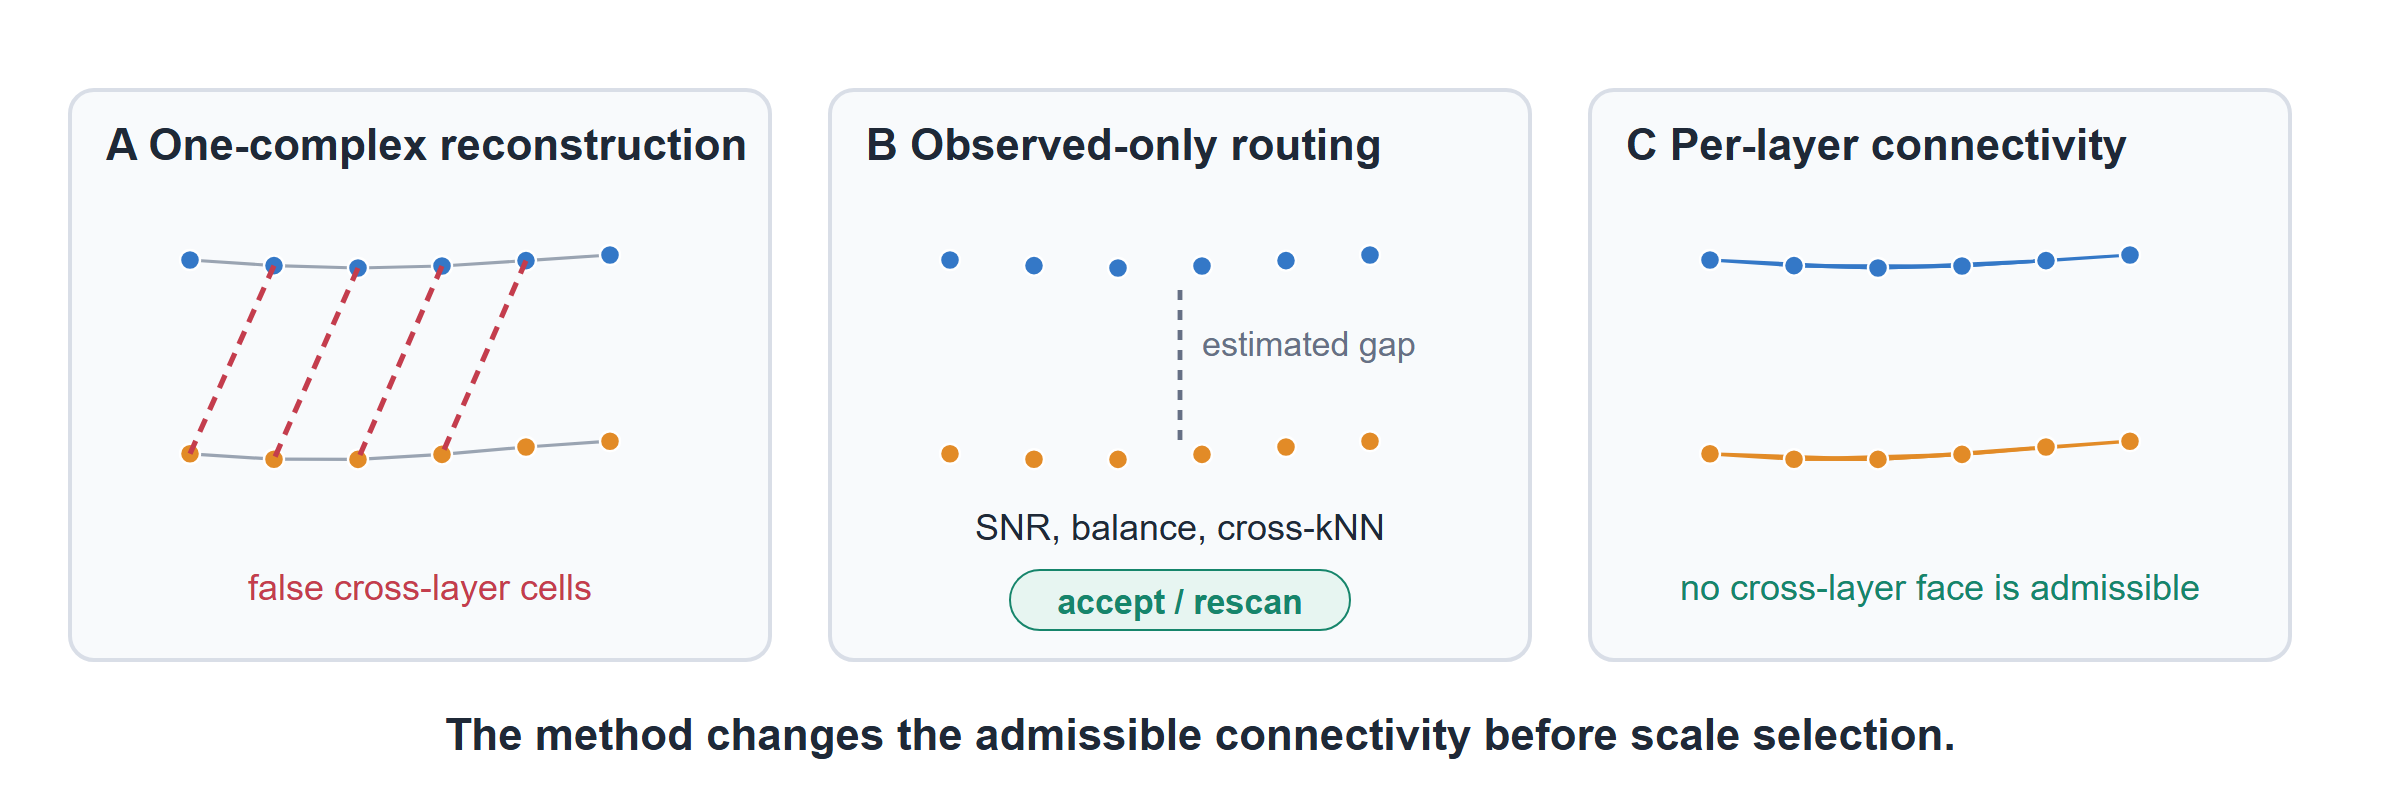
\includegraphics[width=\textwidth]{two_layer_workflow.png}
  \caption{Layer-first 재구성의 핵심. 하나의 3차원 complex는 두 층 사이의
  잘못된 cell을 만들 수 있다(A). 관측 좌표만으로 층 분리와 sampling
  sufficiency를 검사한다(B). 통과한 경우 각 층을 따로 삼각분할하므로 층을
  가로지르는 face는 허용되지 않는다(C).}
  \label{fig:workflow-kr}
\end{figure}

\section{방법}

\subsection{관측 좌표만을 이용한 두 층 추론}

관측 점군을 $X=\{\mathbf{x}_i\}_{i=1}^{n}\subset\mathbb{R}^3$라 하자. 각
점에서 $k=12$개의 최근접 이웃을 이용해 local PCA normal
$\mathbf{n}_i$를 계산한다. Normal은 부호가 반대여도 같은 평면 방향을
나타내므로, 단순 평균 대신 다음 orientation tensor를 사용한다.
\begin{equation}
 \mathbf{Q}=\frac{1}{n}\sum_{i=1}^{n}\mathbf{n}_i\mathbf{n}_i^{\mathsf T},
 \qquad
 \widehat{\mathbf{n}}=\operatorname*{arg\,max}_{\|\mathbf{v}\|=1}
 \mathbf{v}^{\mathsf T}\mathbf{Q}\mathbf{v}.
 \label{eq:normal-kr}
\end{equation}
$\mathbf{Q}$는 ``각 local plane이 공통으로 법선이라고 말하는 방향''을
찾는다. 중심을 뺀 점을 이 방향에 투영해
$h_i=(\mathbf{x}_i-\bar{\mathbf{x}})^{\mathsf T}\widehat{\mathbf{n}}$를 만들고,
결정적인 two-means 반복으로 낮은 층과 높은 층을 나눈다.

두 표면이 함께 완만하게 휘는 합성 조건에서는 shared-trend 변형을 사용한다.
공통 접평면 좌표를 $(u,v,h)$라 하고, 다음의 2차 높이 trend를 두 층이
공유한다고 둔다.
\begin{equation}
 q(u,v)=\beta_0+\beta_1u+\beta_2v+\beta_3u^2+
          \beta_4uv+\beta_5v^2.
 \label{eq:trend-kr}
\end{equation}
Layer label과 $q$를 번갈아 추정한 뒤 residual $h-q(u,v)$의 두 mode로 층을
나눈다. 식~\eqref{eq:trend-kr}은 새로운 PFTF 수식이 아니라, 두 층에 공통인
완만한 굽힘을 제거하는 conventional mixture regression이다.

\subsection{Fail-closed routing}

추론 결과가 믿을 만한지는 세 가지 관측량으로 검사한다. 첫째, 더 작은
cluster의 비율이 0.20 이상이어야 한다. 둘째, 두 층 center 사이의 간격이
각 층 residual spread보다 충분히 커야 한다.
\begin{equation}
 \mathrm{SNR}=\frac{|\mu_1-\mu_0|}
 {\sqrt{n^{-1}\sum_i(r_i-\mu_{z_i})^2}}.
 \label{eq:snr-kr}
\end{equation}
여기서 $z_i$는 추론한 layer이고 $r_i$는 normal height 또는 trend를 뺀
height다. 셋째, 각 점의 $k$-NN 중 다른 layer label을 가진 이웃의 비율인
cross-kNN fraction이 0.05 이하여야 한다. 이 값이 작다는 것은 층 사이보다
한 층 내부의 표본 간격이 더 촘촘하다는 뜻이다.

최종 confirmatory protocol의 SNR 기준은 3.0이다. 두 mode를 식별할 수 없으면
\texttt{unsupported}, 식별은 되지만 sampling이 부족하면
\texttt{rescan\_required}, 구성 결과가 추론한 두 성분을 위반하면
\texttt{algorithm\_failure}로 fail-closed한다. 모든 gate를 통과한 경우에만
\texttt{accept}한다. 정답 layer는 이 판단에 사용하지 않고 false-safe 여부를
평가할 때만 사용한다.

\subsection{층별 constrained connectivity}

각 추론 layer $\ell$의 점을 독립적으로 중심화하고, 가장 큰 두 PCA 축으로
투영한 뒤 2D Delaunay를 계산한다.
\begin{equation}
 \mathcal{T}_{\mathrm{layer}}
 =\mathcal{D}_{2}(\Pi_0 X_0)\cup\mathcal{D}_{2}(\Pi_1 X_1),
 \qquad X_0\cap X_1=\varnothing.
 \label{eq:construction-kr}
\end{equation}
$\Pi_\ell$은 layer의 접평면 투영이고 $\mathcal{D}_2$는 planar Delaunay다.
두 triangle 집합은 원래 3차원 점 index로 되돌려 합치지만 서로 다른 layer를
가로지르는 edge나 face는 추가하지 않는다. 식~\eqref{eq:construction-kr}은
$\alpha$ 값을 최적화하는 식이 아니다. 더 근본적으로 가능한 연결의 집합을
제한한다.

\subsection{Comparator와 endpoint}

B5는 local PCA normal과 density normalization을 사용하는 고정된
anisotropic alpha filtration이다. M1은 density weight로 regular
triangulation의 연결을 바꾸고 proper power circumradius로 score하는 weighted
alpha다. 두 comparator의 scale과 parameter는 confirmatory endpoint와
독립적으로 동결했다.

Geometry endpoint는 고정 거리 tolerance의 surface F-score와, normalized
squared Chamfer 및 Hausdorff를 더한 geometry loss다. F-score는 높을수록,
loss는 낮을수록 좋다. Topology error는 component error, Betti-number error,
정답 layer 사이의 bridge edge와 bridge face를 합한 protocol 지표다.
Nonmanifold edge도 별도로 검사한다. 두 panel은 reference와 sample budget이
다르므로 topology error의 절대 크기는 같은 panel 안에서만 비교한다.

\section{동결 실험 설계}

\subsection{Phase 50 합성 confirmatory panel}

합성 panel은 point count 160/256, control 및 upper occlusion, 75:25 layer
imbalance, anisotropic noise, sinusoidal common trend, local bump의 여섯 stress,
각 12개 repeat로 총 144 case다. 각 case의 observed/reference에 같은 proper
3D rotation을 적용한다. Reference는 4,096점이고 surface endpoint는 1,024개
mesh sample로 계산한다. 사전 gate는 candidate false-safe 0, 전체 safe
coverage 95\% 이상, 각 subgroup 90\% 이상, B5/M1 대비 mean F-score margin
각 0.10 이상, casewise win 75\% 이상, 더 낮은 geometry loss, topology error
0 및 global-normal base 개선이다.

\subsection{S3DIS Area-5 real held-out panel}

S3DIS Areas 1/2/3/4/6에서 floor--ceiling eligibility와 추출 규칙을
보정했다. 다른 건물인 Area 5는 final protocol 및 evaluator commit 전까지
ZIP member name과 size 외의 point 내용을 열지 않았다. 고정 extractor는 한
방의 모든 floor instance와 모든 ceiling instance를 각각 합친다.
Eligibility는 normal angle $\leq5^{\circ}$, projected bounding-box overlap
$\geq0.75$, common footprint에서 layer당 점 수 $\geq592$, gap/plane-residual
SNR $\geq10$, p95 plane residual/median spacing $\leq10$이다.

적격 room을 수동 선택 없이 사전식으로 모두 열거한다. Common footprint에서
각 layer당 관측점 80개와 서로 겹치지 않는 reference 최대 512개를 coordinate
hash로 나눈다. 모든 방법에 같은 normalized $10^{-4}$ general-position
joggle을 적용한다. Area 5를 한 번 연 결과 63개 room이 적격이었다. Gate는
false-safe 0, safe coverage 0.90 이상, B5/M1 availability, mean F-score
margin +0.20/+0.30 이상, casewise win 85\% 이상, 더 낮은 geometry loss,
comparator의 1/4 이하 topology error 및 global-normal ablation non-inferiority다.

\section{결과}

\begin{table}[t]
\centering
\caption{동결 confirmatory 결과. Geometry loss와 topology error는 낮을수록
좋다.}
\label{tab:results-kr}
\footnotesize
\setlength{\tabcolsep}{3pt}
\begin{tabular}{p{0.17\textwidth}p{0.28\textwidth}rrr}
\toprule
Panel & Method & Mean F-score & Geometry loss & Topology error \\
\midrule
Synthetic (144) & Layer-routed & \textbf{0.898536} & \textbf{0.126043} & \textbf{0} \\
 & B5 PCA-anisotropic alpha & 0.515603 & 0.140552 & 45,606 \\
 & M1 weighted power-alpha & 0.620140 & 0.137152 & 11,925 \\
\addlinespace
S3DIS Area 5 (63) & Layer-routed & \textbf{0.805611} & \textbf{0.116385} & \textbf{0} \\
 & B5 PCA-anisotropic alpha & 0.420983 & 0.243356 & 5,214 \\
 & M1 weighted power-alpha & 0.323764 & 0.228920 & 13,375 \\
\bottomrule
\end{tabular}
\end{table}

합성 panel에서 candidate의 mean F-score margin은 B5 대비 +0.382933, M1 대비
+0.278396이고 각각 144/144 case에서 승리했다. 12개의 모든 point-count--stress
subgroup가 12/12 safe accept였다. Global-normal base는 safe accept 138/144,
false-safe 6건이지만 shared-trend candidate는 여섯 사례를 모두 repair해
144/144 safe accept, false-safe 0, nonmanifold edge 0을 달성했다.

S3DIS Area 5에서는 B5 대비 +0.384627, M1 대비 +0.481847의 mean F-score
margin과 각각 63/63 casewise win을 얻었다. Candidate는 62/63 room을 안전하게
수락하고 false-safe가 없었다. 보수적으로 rescan을 요구한 유일한
\texttt{Area\_5/hallway\_5}도 실제 topology는 안전했고 F-score가 0.989640이었다.
B5와 M1은 모든 room에서 구성 가능했다. 모든 panel, safety, construction,
geometry, topology 및 ablation gate가 통과했다(그림~\ref{fig:results-kr}).

\begin{figure}[t]
  \centering
  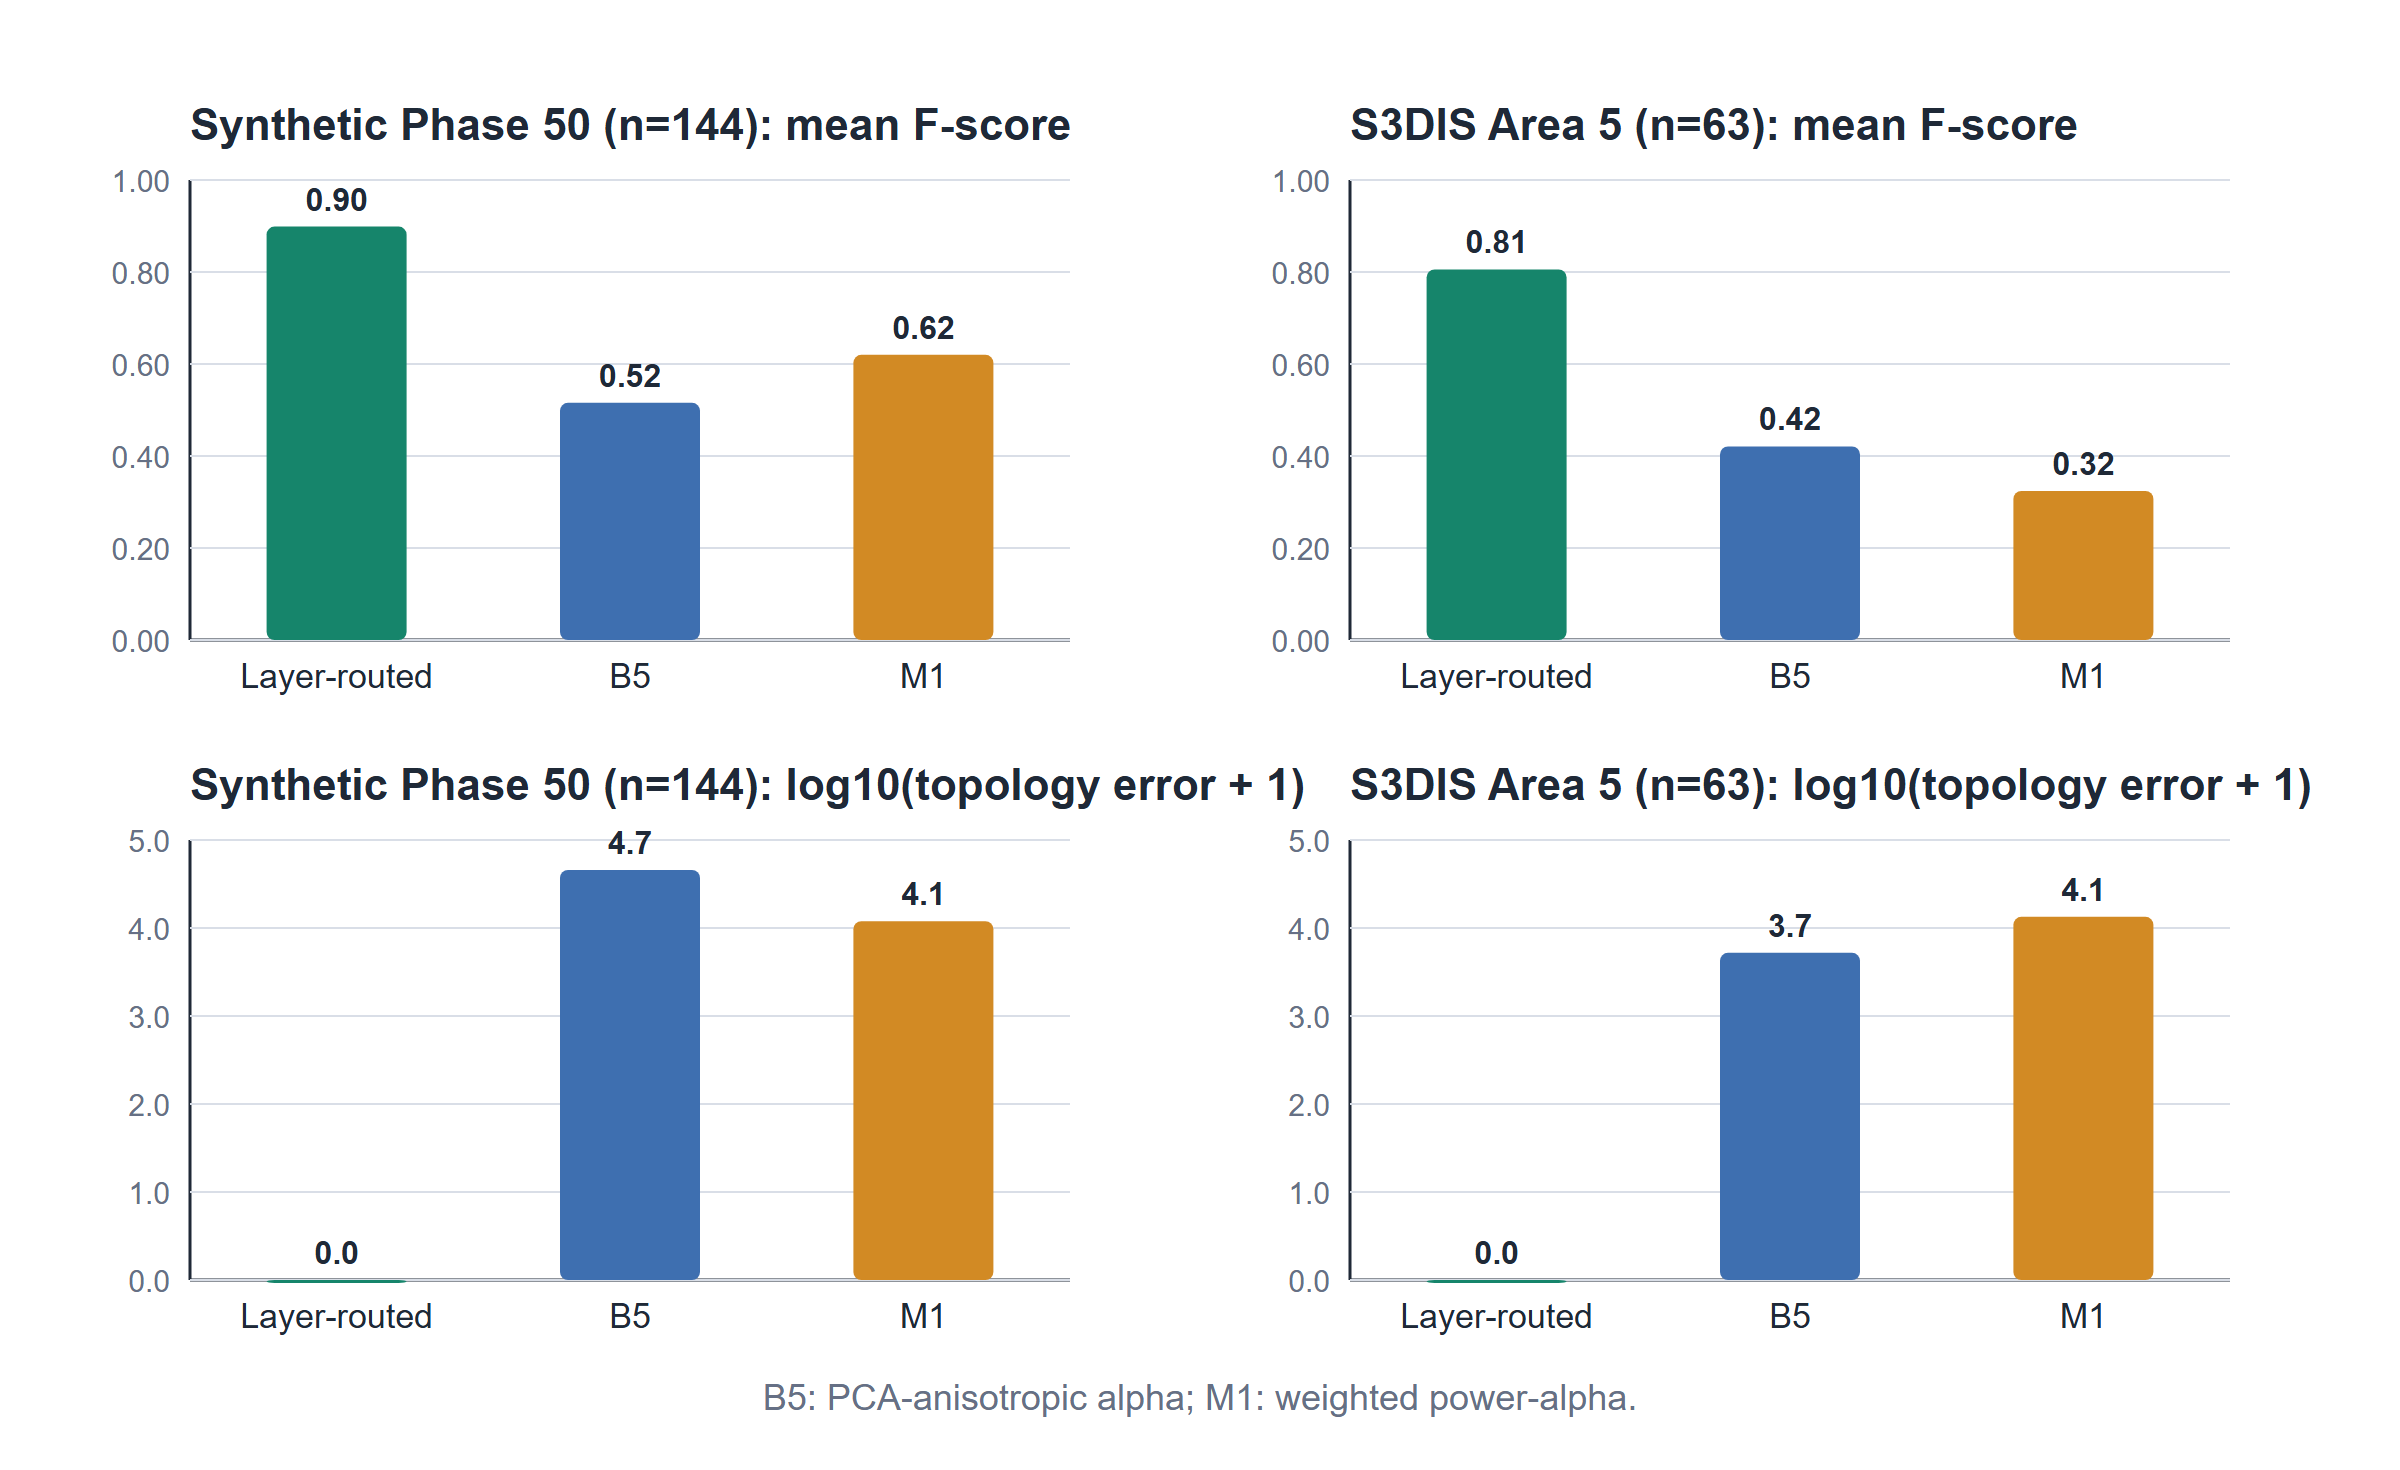
\includegraphics[width=\textwidth]{two_layer_results.png}
  \caption{동결 JSON에서 직접 생성한 결과. 아래 topology panel은 표시를 위해
  $\log_{10}(\mathrm{error}+1)$을 사용하며, 표~\ref{tab:results-kr}에 raw total을
  제시했다.}
  \label{fig:results-kr}
\end{figure}

중요한 ablation 결과가 하나 있다. S3DIS에서 global-normal model은 candidate와
같은 62/63 safe coverage, false-safe 0, 그리고 표시 정밀도에서 같은 mean
F-score를 보였다. 그러므로 실제 데이터의 positive result를 shared-trend의
우월성으로 해석하면 안 된다. 실제 결과가 지지하는 것은 ``두 층을 관측으로
나누고, 통과 여부를 보수적으로 판단하고, 층별로 따로 연결한다''는 전체
구조다.

\section{토론}

큰 개선의 이유는 후보가 alpha의 score만 바꾼 것이 아니라 가능한 연결의
공간을 바꿨기 때문이다. B5는 local metric을 바꾸고 M1은 regular
triangulation을 바꾸지만, 두 방법 모두 두 표면의 합집합을 하나의 3차원
complex로 처리한다. Layer-first 방법은 ``두 개의 식별 가능한 layer''라는
관측 조건을 이용해 문제를 두 개의 planar reconstruction으로 분해한다.
따라서 cross-layer face는 높은 penalty를 받는 나쁜 후보가 아니라 존재할 수
없는 후보가 된다. 본래 질문이었던 alpha selection 문제에 대해, 이 제한된
regime에서는 더 좋은 $\alpha$보다 admissible connectivity가 더 중요하다는
답을 준다.

검증 절차는 결과를 본 뒤의 낙관적 tuning을 줄였다. 합성 parameter와 gate는
untouched arbitrary-pose panel 전에 고정했다. S3DIS에서는 여러 calibration
building으로 eligibility와 split 규칙을 만든 뒤, Area 5를 자동 열거된 하나의
panel로 한 번만 열었다. Candidate decision은 combined XYZ만 사용했다.
Semantic annotation, reference, true layer label은 corpus extraction과
evaluation에만 사용했다. 두 comparator에 대해 207/207 casewise win이므로,
평균 개선이 소수 outlier case 때문인 것도 아니다.

그러나 적용 범위는 명확히 좁다. S3DIS panel은 넓게 겹치는 footprint와
residual/spacing 대비 큰 간격을 가진 거의 평행한 floor--ceiling pair만
포함한다. Close wall--board calibration에서는 geometry 개선이 있었지만,
occlusion으로 두 surface의 실제 관측 support가 겹치지 않아 현재 topology-safe
route가 모두 거부했다. Intersecting surface, 심한 spatial outlier, 합성 N<160,
임의의 multi-surface scene, automatic semantic pair discovery는 검증하지 않았다.
또한 층 내부의 큰 hole이나 복잡한 boundary를 복원하는 단계가 없고,
floating-point Delaunay를 사용하므로 exact 또는 deployment certificate가
아니다.

다음 연구는 세 방향이 적절하다. 첫째, close occlusion을 위해 visibility-aware
support를 추가해야 한다. 둘째, 불완전 footprint에는 boundary-aware planar
meshing 또는 layer 내부 alpha restriction이 필요하다. 셋째, 실제 deployment
평가에는 자동 layer-pair discovery, sensor artifact, runtime/memory 및 exact
또는 host-validated predicate가 포함되어야 한다. 이 후속 문제가 남아 있어도
현재의 좁은 positive claim은 유지된다. Long-gap two-layer 영역에서 동결된
두 독립 confirmatory test가 이미 같은 방향의 결과를 보였기 때문이다.

\section{결론}

충분히 분리된 두 표면 점군에서는 alpha threshold를 계속 조정하는 것보다
연결 가능한 점 쌍을 먼저 제한하는 것이 효과적이었다. Observed-only
fail-closed route와 독립적인 per-layer triangulation은 합성에서 0.279--0.383,
building-disjoint S3DIS에서 0.385--0.482의 mean F-score margin을 얻었고,
두 동결 comparator에 대해 총 207/207 사례에서 승리했으며 aggregate topology
error가 0이었다. 실제 ablation은 이 성공을 shared-trend 또는 PFTF/local-SPD
novelty로 설명할 수 없음을 보여 준다. 최종 결론은 좁지만 긍정적이다. 서로
거의 평행한 두 layer가 관측 좌표에서 식별 가능하고 sampling이 충분한 경우,
두 layer를 따로 재구성하면 그 합집합에 anisotropic 또는 weighted alpha를
적용하는 것보다 정확하고 topology가 안전하다.

\begin{thebibliography}{9}

\bibitem{armeni2016}
I. Armeni, O. Sener, A. R. Zamir, H. Jiang, I. Brilakis, M. Fischer, and
S. Savarese, ``3D Semantic Parsing of Large-Scale Indoor Spaces,''
\emph{Proceedings of the IEEE Conference on Computer Vision and Pattern
Recognition}, pp. 1534--1543, 2016.

\bibitem{edelsbrunner1992}
H. Edelsbrunner, ``Weighted Alpha Shapes,'' Technical Report
UIUCDCS-R-92-1760, University of Illinois at Urbana--Champaign, 1992.

\bibitem{edelsbrunner1994}
H. Edelsbrunner and E. P. M\"ucke, ``Three-Dimensional Alpha Shapes,''
\emph{ACM Transactions on Graphics}, vol. 13, no. 1, pp. 43--72, 1994.

\bibitem{teichmann1998}
M. Teichmann and M. Capps, ``Surface Reconstruction with Anisotropic
Density-Scaled Alpha Shapes,'' \emph{Proceedings of IEEE Visualization '98},
pp. 67--72, 1998, doi:10.1109/VISUAL.1998.745286.

\end{thebibliography}

\end{document}
